\begin{paper}{1}
\begin{header}
\title{Interaction of neutral atoms and homopolar binding according to the quantum mechanics.}
\author{W. Heitler \& F. London}
\location{Zurich}
\note{Presented to the local meeting of the Freiburg German Physical Society in Breisgau, June 12th, 1927. Received June 30th 1927.}
\makeheader
\end{header}
\newcommand{\angstrom}{\mbox{\normalfont\AA}}
\renewcommand{\H}{\El{H}}
\newcommand{\He}{\El{He}}


\begin{abstract}
The play of forces between neutral atoms shows a characteristic quantum-mechanical \?{multiplicity}{Mehrdeutigkeit}. This multiplicity seems suited to understand the various kinds of behavior given in experiments: e.g. in hydrogen the possibility of a homopolar bond resp. an elastic reflection, in the noble gasses on the contrary only the latter -- and indeed this already as a first-order effect of roughly the correct value. In the selection and discussion of the various kinds of behavior the Pauli principle also holds in application to systems of several atoms.
\end{abstract}

The theoretical treatment of the interaction between neutral atoms has up to now caused considerable difficulties. While there has long been a simple picture of the attractive forces of ions, the behavior of neutral atoms, in particular the possibility of a nonpolar binding, has been extraordinarily difficult to understand if one does not resort to very artificial explanations\footnote{For literature on this, see e.h. Handbuch der Physik, vol XXII, 1926, Herzfeld's article.}. 

The development of the quantum mechanics has supplied a totally new viewpoint for the treatment of this problem: first, in the new "model", the charge distribution is of a completely different type\footnote{The correspondence between classical and quantum mechanical quantities relates only to the electrical moments, i.e. to the center of mass of the charge, not to the charge distribution itself, a distinction which cannot be resolved by the usual spectroscopic questions.} than in the Bohr model (namely, falling off as $\exp{-r}$), which would already cause a totally different set of forces between "neutral" atoms. But more essential, and decisive for the understanding of the possible types of behavior between neutral atoms, proves to be a characteristic quantum-mechanical \?{beat phenomenon}{Schwebungsphänomen}, which is similar to the \?{resonance beats}{Resonanzschwebungen} found by Heisenberg. We will study as an example of this behavior two \El{H}-atoms (\S1) as well as two \El{He}-atoms (\S3). To anticipate the result (\S2): two solutions are obtained for the interaction energy: One, which gives attraction at moderate distances and repulsion at small distances, and which is suitable for the formation of a homopolar molecular (even at first order, in which perturbations from polarization are ignored). This solution is however not allowed for \El{He} in the ground state because of the Pauli principle (\S4). A second solution, which comes into play in \El{He} alone, gives repulsion everywhere (van der Waals' $b$-force).

\section{Interaction of two hydrogen atoms.} We now set for ourselves the task of determining the change in energy experienced by two ground-state hydrogen atoms, if we bring them to a distance $R$ (measured as the distance between the nuclei). According to whether this additional energy decreases or increases with the gradual approach of the atoms, we find\footnote{It is not superfluous to draw attention to the fact that the connection assumed here between wave-mechanical frequency and mechanical energy is absolutely hypothetical, since we know that the Lorentz force law that determines the effect of the field on matter is replaced in quantum mechanics by a totally different one, namely the wave equation.} attraction or repulsion.

\subsection{} We denote the two nuclei, whose mutual distance is fixed once and for all and is equal to $R$, with $a$ and $b$, the two electrons with the numbers 1 and 2, finally the distances of the electrons from the nuclei and from one another by $r_{a1}, \dots, r_{12}$.

The wave equation of our problem -- the 2-hydrogen-atom-problem -- then reads $\left(\text{with } \Delta_{12}=\Delta_1+\Delta_2=\ppX{}\ppY{x_1} + \ppX{}\ppY{y_1} + \ppX{}\ppY{z_1} + \ppX{}\ppY{x_2} + \ppX{}\ppY{y_2} + \ppX{}\ppY{z_2}\right)$:

\nequ{1}{
(\chi)\equiv \Delta_{12}\chi + \frac{8\pi^2 m}{h^2}\left\{
E - \left(\frac{\varepsilon^2}{R} + \frac{\varepsilon^2}{r_{12}} - \frac{\varepsilon^2}{r_{a1}} - \frac{\varepsilon^2}{r_{a2}} - \frac{\varepsilon^2}{r_{b1}} - \frac{\varepsilon^2}{r_{b2}}\right)\right\}\chi = 0.
}

We are interested in those solutions $\chi$ which correspond to the perturbation of two neutral \El{H}-atoms in the ground state, and accordingly we will initially approximate them with the well-known eigenfunctions of the hydrogen ground state.

If electron 1 is at nucleus $a$, then then it is assigned to the well-known hydrogen eigenfunction
\nequ{2}{
\psi(1) = \frac{1}{\sqrt{\pi}}\left(\frac{1}{a_0}\right)^{3/2}\exp{-\frac{r_{a1}}{a_0}},
}
where $a_0$ denotes the Bohr radius of the $1_1$-orbit. The argument $1$ identifies the coordinates of the electron 1 in the $q$-space, so in the future we write it as an index $\psi_1$ (swapping the eigenvalue index is not to be feared, since we always consider atoms in the ground state). Accordingly
\nequ{2'}{
\varphi_1 = \frac{1}{\sqrt{\pi}}\left(\frac{1}{a_0}\right)^{3/2}
\exp{-\frac{r_{b1}}{a_0}}
}
denotes the first electron being found at nucleus $b$. The two eigenfunctions (2) and (2') are completely different if they can also be \?{brought into alignment}{zur Deckung gebracht} by a simple translation\footnote{Accordingly one might in the following always keep in mind that our conclusions remain unchanged even if $\psi$ and $\varphi$ differ in their form, whereby our considerations can immediately be stretched to a fundamentally more general region of application.}; then they act in different regions of space.

Corresponding eigenfunctions exist for electron 2:
\nequ{2a}{
\psi_2 = \frac{1}{\sqrt{\pi}}\left(\frac{1}{a_0}\right)^{3/2}\exp{-\frac{r_{a2}}{a_0}},\quad
\varphi_2 = \frac{1}{\sqrt{\pi}}\left(\frac{1}{a_0}\right)^{3/2}\exp{-\frac{r_{b2}}{a_0}},
}
which state that the electron 2 is found at the nucleus $a$ resp. $b$. The eigenfunctions (2a) are different from the eigenfunctions (2) and (2') only in the $q$-space.

\subsection{} As unperturbed eigenfunctions we have to choose those which state that one\footnote{For now we exclude the possibility of ionization; how far this is justified will only be shown later in \S5.} electron is found at one nucleus, the other electron at the other nucleus. In these two still-uncoupled systems are taken together as one system, it is known that the product of these two eigenfunctions is to be taken as the common eigenfunction. But that is possible in two different ways -- according to the distribution of the two electrons on the two nuclei. At first:
\nequ{3a}{
\psi_1\varphi_2\quad \text{(1 is at $a$, 2 is at $b$)}.
}
But one could just as well have:
\nequ{3b}{
\psi_2\varphi_1\quad \text{(2 is at $a$, 1 is at $b$)}.
}

Both possibilities are associated with the same energy for the total system (double the hydrogen energy). This is a case of twofold degeneracy: all pairs of orthogonal linear combinations of $\psi_1\varphi_2$ and $\psi_2\varphi_1$:
\nequ{4}{
\alpha &= a\psi_1 \varphi_2 + b\psi_2 \varphi_1\\
\beta &= c\psi_1 \varphi_2 + d\psi_2 \varphi_1\\
}
with the normalization and orthogonality conditions
\nequ{5}{
\begin{array}{lrl}
a^2+b^2+& 2abS &=1,\\
c^2+d^2+& 2cdS &=1,\\
ac + bd+& (ad+bc)S &=0
\end{array}
}
(where $S=\int\psi_1\varphi_1\psi_2\varphi_2\d\tau_1\d\tau_2$) are regarded as unperturbed eigenfunctions of the problem.

\subsection{} The exact eigenfunctions of the differential equation (1) emerge from totally determinate linear combinations (4), the "zero-order" eigenfunctions and are distinguished from the latter only by a small perturbation $v$. The coefficients $a,b,c,d$ in (4) for these zero-order eigenfunctions can by determined according to well-known rules. Though equation (1) lacks the character of a perturbation problem, since no part of the potential function can be separated off as a "perturbation potential", the method of determining the desired coefficients and the perturbation energies is still just the same as if a perturbation potential were present. In order to make the calculations more transparent, we will from the outset select the correct linear combinations, normalized according to (5) (and their correctness will be verified later):
\nequ{4a}{
\alpha &= \frac{1}{\sqrt{2+2S}}(\psi_1\varphi_2+\psi_2\varphi_1),\\
\beta  &= \frac{1}{\sqrt{2-2S}}(\psi_1\varphi_2+\psi_2\varphi_1).
}
For the perturbed eigenfunctions we will now have to suppose
\nequ{6}{
\chi_\alpha &= \alpha + v_\alpha,\\
\chi_\beta &= \beta + v_\beta.
}
With this \textit{Ansatz} we go into equation (1) and note that the functions $\psi_1,\psi_2,\varphi_1,\varphi_2$ satisfy the four equations
\nequ{7}{
\Delta_1 \psi_1 + \frac{8\pi^2 m}{h^2}\left(E_0+\frac{\varepsilon^2}{r_{a1}}\right)\psi_1&=0,\\
\Delta_2 \psi_2 + \frac{8\pi^2 m}{h^2}\left(E_0+\frac{\varepsilon^2}{r_{a2}}\right)\psi_2&=0,\\
\Delta_1 \varphi_1 + \frac{8\pi^2 m}{h^2}\left(E_0+\frac{\varepsilon^2}{r_{b1}}\right)\varphi_1&=0,\\
\Delta_2 \varphi_2 + \frac{8\pi^2 m}{h^2}\left(E_0+\frac{\varepsilon^2}{r_{b2}}\right)\varphi_2&=0,\\
}
where $E_0=-13.5\unit{Volt}$ denotes the eigenvalue of the hydrogen ground state. With the notation
\nequ{8}{
E_1=E-2E_0
}
for the eigenvalue perturbation we obtain from (1) the two differential equations for $v_\alpha$ and $v_\beta$:
\nequ{9$\alpha$}{
\sqrt{2+2S}L(v_\alpha) &+ \left(E_1 - \frac{\varepsilon^2}{r_{12}} - \frac{\varepsilon^2}{R}\right)(\psi_1\varphi_2 + \psi_2\varphi_1)\\
&+ \left(\frac{\varepsilon^2}{r_{a1}} + \frac{\varepsilon^2}{r_{b2}}\right)\psi_2\varphi_1
+ \left(\frac{\varepsilon^2}{r_{b1}} + \frac{\varepsilon^2}{r_{a2}}\right)\psi_1\varphi_2 = 0,
}
\nequ{9$\beta$}{
\sqrt{2-2S}L(v_\beta) &+ \left(E_1 - \frac{\varepsilon^2}{r_{12}} - \frac{\varepsilon^2}{R}\right)(\psi_1\varphi_2 + \psi_2\varphi_1)\\
&+ \left(\frac{\varepsilon^2}{r_{a1}} + \frac{\varepsilon^2}{r_{b2}}\right)\psi_2\varphi_1
- \left(\frac{\varepsilon^2}{r_{b1}} + \frac{\varepsilon^2}{r_{a2}}\right)\psi_1\varphi_2 = 0.
}

In order for this equation that is inhomogeneous in $v$ to be solvable at all for an eigenvalue $E$ of the homogeneous equation, it must be demanded that the inhomogeneities are orthogonal to all the eigenfunctions of the homogeneous equation, thus to $\chi_\alpha$ and $\chi_\beta$ which are associated to the same eigenvalue $E$.

It is first found that the inhomogeneities of ($9\alpha$) are already orthogonal to $\beta$ and the inhomogeneities of ($9\beta$) to $\alpha$ (up to negligible quantities). Hence the correctness of the \textit{Ansatz} (4a) is verified. The two other requirements:
\begin{enumerate}
	\item Inhomogeneities of ($9\alpha$) $\perp$ to $\alpha$,
	\item Inhomogeneities of ($9\beta$) $\perp$ to $\beta$,
\end{enumerate}
supply the two eigenvalue perturbations:
\nequ{10}{
E_\alpha &= E_{11} - \frac{E_{11}S - E_{12}}{1+S},\\
E_\beta  &= E_{11} + \frac{E_{11}S - E_{12}}{1-S}
}
with the following notation:
\nequ{11}{
E_{11} = &\int\left[\left(\frac{\varepsilon^2}{r_{12}}+\frac{\varepsilon^2}{R}\right)\frac{\psi_1^2\varphi_2^2 + \psi_2^2\varphi_1^2}{2} - 
\left(\frac{\varepsilon^2}{r_{a1}}+\frac{\varepsilon^2}{r_{b2}}\right)\frac{\psi_2^2\varphi_1^2}{2}\right.\\
& \quad\quad\left. \left(\frac{\varepsilon^2}{r_{a2}}+\frac{\varepsilon^2}{r_{b1}}\right)\frac{\psi_1^2\varphi_2^2}{2}\right]\d\tau_1\,\d\tau_2,\\
E_{12} =& \int\left(\frac{2\varepsilon^2}{r_{12}} + \frac{2\varepsilon^2}{R}
 - \frac{\varepsilon^2}{r_{a1}} - \frac{\varepsilon^2}{r_{a2}}
 - \frac{\varepsilon^2}{r_{b1}} - \frac{\varepsilon^2}{r_{b2}}
\right)\frac{\psi_1\varphi_1\psi_2\varphi_2}{2}\d\tau_1\,\d\tau_2,\\
S =& \int\psi_1\varphi_1\psi_2\varphi_2 \d\tau_1\,\d\tau_2.
}

\section{Discussion of the results.}
\subsection{} Thus we obtain two perturbation energies corresponding to the \textit{Ansatzes} (5a):
\uequ{
E_\alpha &= E_{11} - \frac{E_{11}S - E_{12}}{1+S}
}
associated with $\frac{1}{\sqrt{2+2S}}(\psi_1\varphi_2+\psi_2\varphi_1)$ (symmetric in 1 and 2),
\uequ{
E_\beta  &= E_{11} + \frac{E_{11}S - E_{12}}{1-S}
}
associated with $\frac{1}{\sqrt{2-2S}}(\psi_1\varphi_2-\psi_2\varphi_1)$ (antisymmetric in 1 and 2).

It is a result that can only be described very artificially with classical concepts that two neutral atoms can interact with one another in two different ways.  We are probably not far away from an actual understanding of this matter. But it is desirable to at least clarify how this remarkable \?{ambiguity}{Zweideutigkeit} comes about mathematically. The essential thing is obviously that the problem is originally twofold degenerate (1a and 1b), corresponding to the two possibilities of assigning the electrons among the neutral atoms\footnote{In the classical mechanics, this problem is not degenerate; the same energy value is indeed associated to the two electron assignments. But the criterion for degeneracy in the classical mechanics is not $E_k-E_l=0$, but rather $\nu\equiv\pX{E}\pY{J}=0$ (A "\?{neighborly relationship}{Nachbarschaftsbeziehung}" as regards the action variable $J$). Actually, even in this case the electrons have their full degree of periodicity. Only when the energy is sufficient to overcome the potential barrier between the two atoms (or at a sufficient distance from both the atoms) does $E_k-E_l=0$ have $\pX{E}\pY{J}=0$ as a consequence and the problem is degenerate. With that the electrons now describe orbits about both nuclei and are constantly \?{exchanging places}{tauschen sich aus}. This distinction does not occur in the quantum mechanics (cf F. Hund, ZS. f. Phys. 40, 442, 1926). With even greater (finite) potential wells there is accordingly always a certain probability for an exchange of the electrons. While there is a possibility in classical mechanics of giving the electrons fixed labels (put each electron in a sufficiently deep potential well and withhold any greater supply of energy), something equivalent in quantum mechanics is impossible: even if it is known in one instant than an electron is in one potential well, it is never certain whether in the next instant it hasn't already exchanged with another. Therefore statistics which in principle refrain from any individualization of the electrons and only take into account the numerical distribution in the states -- like the Bose or Fermi statistics -- fit the possible quantum-mechanical descriptions extraordinarily well.}. Lifting this degeneracy is linked with, as is evident from (10), the non-vanishing of the eigenfunction of the atom $a$ at the position of the atom $b$ and conversely (otherwise we would have $\psi_1\varphi_1=0$ and consequently $E_{12}=0$ and $S=0$); but that means that there must exist a finite probability for the electron of $a$ to belong to $b$. The exponential behavior of $\psi$ and $\varphi$ in fact always fulfills this condition. The quantity $1/h(E_\beta - E_\alpha)$ is taken as the mean frequency with which an exchange of the two electrons occurs. For large distances this difference decreases as $\frac{\varepsilon^2}{a_0}\exp{-\frac{2}{a^0}R}$, so that widely-separated atoms only enter into exchange very rarely\footnote{The medium gas-kinetic dimensions ($3.3\cdot 10^{-7}\unit{cm}$) are already "large" distances; there, the period of an exchange is $\frac{a_0}{\varepsilon^2}h\cdot\exp{\frac{2}{a_0}3.3\cdot 10^{-7}} \approx 10^{30} \unit{years}$; on the contrary at the distances in a crystal lattice ($\approx 3\cdot 10^{-8}\unit{cm}$) an exchange \?{lasts}{dauert} $10^{-10}\unit{sec}$.}.

The whole phenomenon is closely related to the quantum-mechaical resonance phenomena treated by Heisenberg. But while in resonance the electrons of different \?{levels of motion}{Bewegungsstufen} of one and the same series of eigenfunctions exchange their energies, here electrons of the same level of excitation (same energy), but different systems of eigenfunctions ($\psi$ and $\varphi$) exchange their positions. There the double occurrence of the same jump frequency is characteristic (resonance phenomenon); here in contrast resonance does not come into play.

\subsection{} Now we turn to the quantitative discussion of the interaction energies (10). Even without evaluating the relevant integrals it can be stated: the sign of $E_{11}S-E_{12}$ is always positive. In a Sturm-Liouville eigenvalue problem of arbitrarily-many dimensions with homogeneous boundary conditions possesses those \?{eigenvibrations}{Eigenschwingungen} of the lowest eigenvalue which have no nodes. Every other orthogonal eigenvibration has nodes and a higher eigenvalue. But now apparently the solution $\alpha$ has no nodes, while $\beta$ as an antisymmetric eigenfunction always has a node. So,
\nequ{12}{
E_\beta>E_\alpha.
}

The meaning of $E_{11}$ is immediately clear from (11): it is the pure Coulomb interaction of the charge distribution that is present. Calculation gives
\nequ{13}{
E_{11} = \frac{\varepsilon^2}{a_0}\exp{-\frac{2}{a_0}R}
\left(\frac{a_0}{R}+\frac{5}{8}-\frac{3}{4}\frac{R}{a_0}-\frac{1}{6}\frac{R^2}{a_0^2}\right).
}
The middle curve in figure 1 shows the course. $R$ given is in units of $a_0=0.532\unit{\AA}$, the energy in \unit{Volts}.

The remaining part of the energies (11) cannot be so simply interpreted. The integrals occurring there cannot all be evaluated. One calculates:
\nequ{14}{
\begin{array}{c}
S=\left(1+\frac{R}{a_0}+\frac{R^2}{3a_0^2}\right)^2\exp{-\frac{2R}{a_0}}\\
\int\frac{\psi_1\psi_2\varphi_1\varphi_2}{2}\left(
\frac{\varepsilon^2}{r_{a1}} + \frac{\varepsilon^2}{r_{a2}} + \frac{\varepsilon^2}{r_{b1}} + \frac{\varepsilon^2}{r_{b2}} - \frac{2\varepsilon^2}{R}
\right)\d\tau_1\,\d\tau_2\\
=\frac{2\varepsilon^2}{a_0}\left(1+\frac{2R}{a_0}+\frac{4}{3}\frac{R^2}{a_0^2}+\frac{R^3}{a_0^3}\right)\exp{-\frac{2R}{a_0}} - \frac{\varepsilon^2}{R}S,
\end{array}
}
while for the missing integral over $1/r_{12}$ we only obtain an upper bound\footnote{It has to do with the self-potential of a charge distribution over confocal ellipsoids, which is much more complicated than the well-known Dirichlet solution for similarly-situated ellipsoids. In the estimate (15) the ellipsoid was replaced by a sphere with the same total charge.}. It is
\nequ{15}{
\frac{\psi_1\psi_2\varphi_1\varphi_2}{r_{12}}\d\tau_1\,\d\tau_2
< \frac{\varepsilon^2}{a_0}\frac{5}{8}\left(1+\frac{R}{a_0}+\frac{R^2}{3a_0^2}\right)^2\exp{-\frac{2R}{a_0}}.
}
\begin{wrapfigure}{L}{0.5\textwidth}
%	\begin{center}
		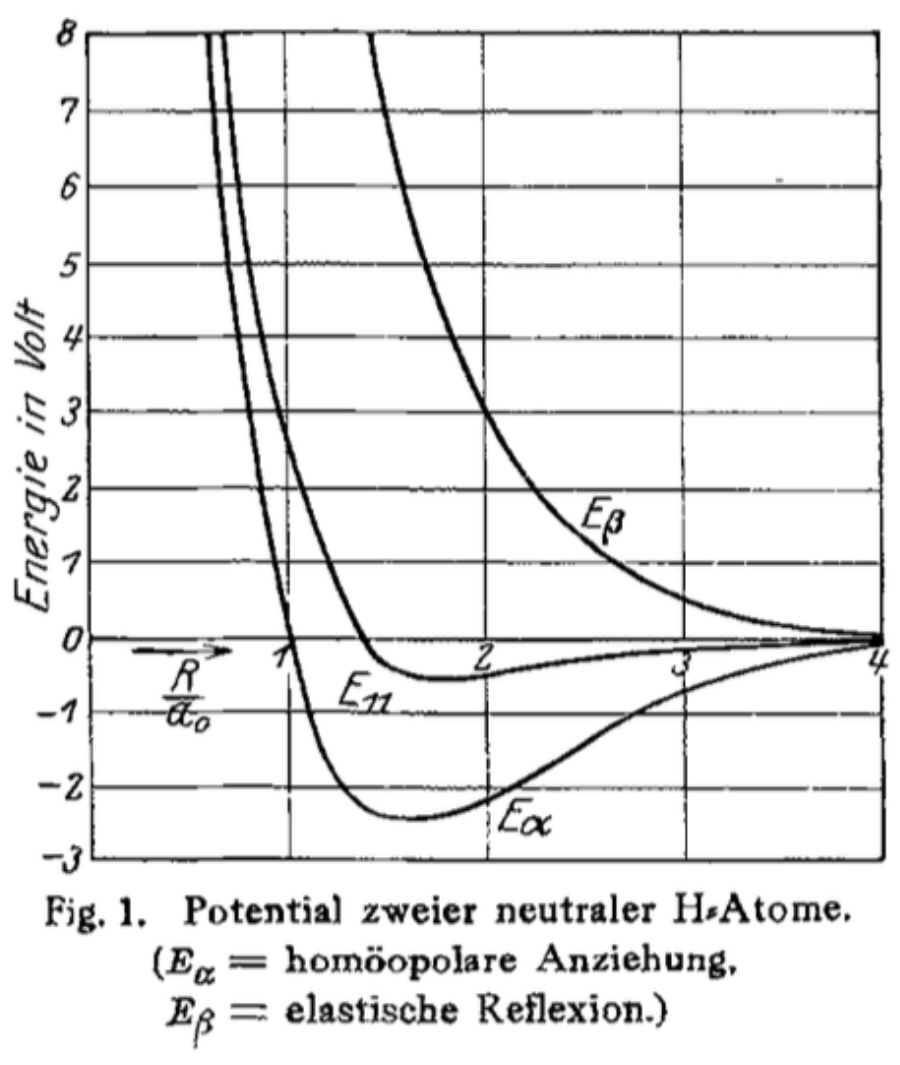
\includegraphics[width=0.5\textwidth]{fig1}
%	\end{center}
\end{wrapfigure}

With this upper limit we get the curves $E_\alpha$ and $E_\beta$ in figure 1.

$E_\beta$ consistently shows repulsion; $E_\alpha$ shows attraction at larger distances, then a minimum approximately at $R=\frac{3}{2}a_0$ and a repulsion at smaller distances. The nonpolar attraction occurring here appears as a characteristic quantum-mechanical effect. It is already present without consideration of the perturbations by polarization. It is also worth noting that the repulsion $E_\beta$, as is seen, is in large part likewise due to this quantum-mechanical effect, not the Coulomb interaction ($E_{11}$).

We claim that the physical meaning of the two solutions is the following: the antisymmetric solution of the interaction energy $E_\beta$ corresponds to the van der Waals repulsion (elastic reflection) of the two hydrogen atoms. If however $\alpha$ is excited, then the two hydrogen atoms could merge into a homopolar molecule, where the minimum of $E_\alpha$ specifies the equilibrium position. We will further show that in the interaction of two non-excited noble gas atoms (\S3) the solution which would correspond to molecule formation is quantum-theoretically forbidden. The reasoning behind this assertion follows in \S4.

The approximate curves roughly give the values of the relevant atomic quantities: atomic diameter, dissociation energy and moment of inertia of the molecule. As to the errors brought about by the estimation, it is noted that in every case $E_\beta$ is actually higher, $E_\alpha$ lower, whereby the typical character of the two potentials would then be even more strongly expressed. Since it is not our goal to work out the most exact numerical values possible, but rather to get a view into the physical behavior of the homopolar binding, this estimate will suffice us here.

\section{Interaction of two \El{He} atoms} We investigate with the same method the interaction of two neutral \El{He} atoms. The two nuclei are again called $a$ and $b$ and are held at a fixed distance $R$. The electrons have the numbers 1 through 4. For each nucleus there is an eigenfunction, $\psi$ for the nucleus $a$, $\varphi$ for the nucleus $b$. which are each now however functions of two electrons, and indeed Heisenberg's \El{He} theory\footnote{W. Heisenberg, ZS. f. Phys. 38, 411, 1926} has shown that the eigenfunctions of the \El{He} ground state are symmetric in the position coordinates of the two electrons. By forming products with one $\psi$-function and one $\varphi$-functions an eigenfuncton of the unperturbed problem emerges (we again write the arguments as indices):
\nequ{16}{
\psi_{ik}\cdot\varphi_{lj}\quad (i\neq j\neq l\neq j=1,2,3,4)
}
(widely separated neutral atoms). By permuting the four electrons (taking into account that $\psi_{ik}=\psi_{ki}$ and $\varphi_{ik}=\varphi_{ki}$) there arise 6 new eigenfunctions which are all associated to the same eigenvalue. They are
\nequ{17}{
\begin{array}{ll}
	\psi_{12}\varphi_{34}, & \psi_{34}\varphi_{12},\\
	\psi_{13}\varphi_{42}, & \psi_{42}\varphi_{13},\\
	\psi_{14}\varphi_{23}, & \psi_{23}\varphi_{14}.
\end{array}
}
The electrons of the helium ground state must be different from one another with respect to their \?{spin}{Dralls}. We will choose the notation so that the electrons 1 and 3 have the same spin, likewise 2 and 4 but 1 and 2 have different spin. Then, according to the Pauli principle it is forbidden for 1 and 3 resp. 2 and 4 to be found at the same \El{He} nucleus. We could consequently exclude two of the six eigenfunctions (17) from the outset and limit ourselves to
\nequ{17a}{
\begin{array}{ll}
	\psi_{12}\varphi_{34}, & \psi_{34}\varphi_{12},\\
	\psi_{14}\varphi_{23}, & \psi_{23}\varphi_{14}.
\end{array}
}
The wave equation for the 2-\El{He} problem reads
\nequ{18}{
\sum\limits_{i=1}^4\left[\Delta_i\chi + \frac{8\pi^2m}{h^2}\left(
E-\varepsilon^2\left(\frac{4}{R}+\sum\limits_{k=1}^4\frac{1}{r_{ik}} - 
\frac{1}{r_{ai}}-\frac{1}{r_{bi}}\right)\right)\chi
\right] = 0.
}

It is symmetric in all four electrons. Here again we do not have a perturbation problem of the usual form, since as in \S1 no perturbing potential can be separated off; but we gather from the symmetry of the differential equation that the zero-order eigenfunctions are the same as if a small perturbing potential that is symmetric in the four electrons were present. We denote it with $H$.

With this we could of course not derive the first-order eigenvalues from the secular problem, though we can derive the correct zero-order eigenfunctions if these alone are distinguished by the symmetry character of the differential equation. Instead of dealing with the secular problem with $H$ with the eigenfunctions (17a), it is more practical to from the outset form certain linear combinations of (17a), namely (we leave off the normalization factors):
\nequ{17b}{
\begin{array}{ll}
\Psi_1 = \psi_{12}\varphi_{34} + \psi_{34}\varphi_{12}, &
\Phi_1 = \psi_{12}\varphi_{34} - \psi_{34}\varphi_{12}, \\
\Psi_2 = \psi_{14}\varphi_{23} + \psi_{23}\varphi_{14}, &
\Phi_2 = \psi_{14}\varphi_{23} - \psi_{23}\varphi_{14}. \\
\end{array}
}

With these eigenfunctions, all matrix elements of the form
\uequ{
\int H\Psi\Phi\d\tau = 0
}
vanish, since $H\Psi$ is symmetric with respect to an exchange of 1 and 3 and simultaneously 2 and 4, while $\Phi$ is antisymmetric, but the integral is insensitive to an exchange in integration variables, so it must vanish. Further, the following matrix elements enter into the secular problem:
\uequ{
\begin{array}{lll}
\int H\Psi_1^2\d\tau &= \int H\Psi_2^2\d\tau &= H_{11},\\
\int H\Psi_1\Psi_2\d\tau &= H_{12},\\
\int H\Phi_1^2\d\tau &= \int H\Phi_2^2\d\tau &= K_{11},\\
\int H\Phi_1\Phi_2\d\tau &= 0.
\end{array}
}

The fourth-degree secular problem for the perturbation energy $E$ then reads:
\uequ{
\begin{array}{r}
	\,\\
	\Psi_1 \\
	\Psi_2 \\
	\Phi_1 \\
	\Phi_2 \\
\end{array}
\begin{array}{rccccl}
	\, &\Psi_1 & \Psi_2 & \Phi_1 & \Phi_2 \\
	\vline &H_{11} - E & H_{12} & 0 & 0 &\vline \\
	\vline &H_{12} & H_{11} - E & 0 & 0 &\vline \\
	\vline &0 & 0 & K_{11} - E & 0 &\vline \\
	\vline &0 & 0 & 0 & K_{11} - E &\vline 
\end{array} = 0
}

One obtains a twofold degenerate eigenvalue $K_{11}$ and rwo non-degenerate eigenvalues:
\nequ{19}{
	E_\alpha \quad\, & = H_{11} + H_{12},\\
	E_\beta \quad\, & = H_{11} - H_{12},\\
	\left.
	\begin{array}{l}
	E_\gamma\\
	E_\delta
	\end{array}\right\} &= K_{11}.
}

Additionally, the zero-order eigenfunctions are found following the well-known procedure:
\nequ{20}{
\begin{array}{lllcl}
	\alpha &= \Psi_1 + \Psi_2 &= \psi_{12}\varphi_{34} + 
	\psi_{34}\varphi_{12} &+& \psi_{14}\varphi_{23} +\psi_{23}\varphi_{14},\\
	\beta &= \Psi_1 - \Psi_2 &= \psi_{12}\varphi_{34} + 
	\psi_{34}\varphi_{12} &-& \psi_{14}\varphi_{23} -\psi_{23}\varphi_{14},\\
	\gamma &= \Phi_1 &= \psi_{12}\varphi_{34} - \psi_{34}\varphi_{12},\\
	\delta &= \Phi_2 &= \, & & \psi_{14}\varphi_{23} - \psi_{23}\varphi_{14}.
\end{array}
}

On the same grounds as in the 2 hydrogen atom problem, $E_0$ must be the lowest eigenvalue, and consequently $H_{12}<0$; since $E_\alpha$ is associated with the node-free symmetric eigenfunction $\alpha$. In the meantime in the following section we will show that this $\alpha$, which would energetically enable molecule formation, is not quantum-theoretically permitted for neutral \El{He}, that rather from the four solutions (20) only $\beta$ can occur, which would again mean elastic reflection.

\section{Pauli principle and molecule formation.} \subsection{} As one is easily convinced, our solutions (4a) resp. (20) belong to systems which do not combine with one another\footnote{They are different from a similar case, recently examined by F. Hund, ZS. f. Phys. 40, 743, 1927, namely the \?{two-center problem}{Zweizentrenproblem} with one electron in which solutions of the form $\varphi+\psi$ and $\varphi-\psi$, which combine with one another.} This circumstance opens up the possibility of applying the Pauli principle, which has proven itself in the  discussion of the electron configuration, in an expanded sense to the system of two interacting systems, in order to get a narrower selection of the quantum-theoretically allowed types of behavior of two atoms.

The following formulation of this rule is sufficient for our purpose\footnote{This formulation of the Pauli principle is not entirely correct. But a really general version of it is still not known. We refer to the work of W. Heisenberg, ZS. f. Phys. 41, 239, 1927, and particularly the upcoming considerations of F. Hund.}: the chosen eigenfunctions of the system should, by swapping two electrons, $\frac{\text{change}}{\text{maintain}}$ their sign when the two electrons have $\frac{\text{the same}}{\text{different}}$ spins. (A so-called "eigenfunction of the spin" is not considered here.)

\subsection{} We apply this rule to the solutions of \S1 and \S3. For hydrogen the symmetric $\alpha$ keeps its sign by swapping 1 and 2, $\beta$ changes it. With $\alpha$ then the two electrons must have different spin, with $\beta$ the same spin. Since however there is no restriction on the spin of separated atoms. both solutions could occur -- each according to chance.

For the solutions (20) of the 2-\El{He} problem however we know that 1 and 3 as well as 2 and 4 have the same spin, on the other hand 1 and 2 as well as 3 and 4 differ. Limits are thereby placed on the \?{permutability}{Vertauschbarkeit} of the electrons from the outset. If the individual \El{He} atoms are to be able to exist (Pauli principle applied to the individual \El{He} atom), then only the electrons 1 and 3 or 2 and 4 may be switched. The chosen eigenfunctions must be antisymmetric with respect to each of these permutations. By permuting both pairs they must be reproduced (without a change of sign). The eigenfunctions $\alpha,\beta,\gamma,\delta$ now go, under the aforementioned permutations, over into
\uequ{
\begin{array}{c||c|c||c}
	\hline\hline
	\, & \text{1 with 3} & \text{2 with 4} & \substack{\text{1 with 3 and}\\\text{ 2 with 4}}\\
	\hline\hline
	\alpha \to & +\alpha & +\alpha & +\alpha\\
	\beta \to & -\beta & -\beta & +\beta\\
	\gamma \to & -\delta & +\delta & -\gamma\\
	\delta \to & -\gamma & +\gamma & -\delta\\
\end{array}
}

So we see that with \El{He}, only the solution $\beta$ satisfies the requirements. It is however associated with the higher eigenvalue. If we carry over the behavior from hydrogen here, then we have to take for the dependence of the interaction on $R$ the upper curve $E_\beta$ from figure 1, which always gives repulsion. Closer discussion shows that it gives roughly the correct magnitude of the gas-kinetic \El{He} radius. The extraordinary restriction that we find here with \El{He} is obviously grounded in the fact that 2 \El{He} atoms (the same goes for all noble gasses) are not distinguishable as regards their spins -- in contrast to hydrogen (and all atoms with unfilled shells) -- whereby for 2 \El{He} atoms only a single type of behavior is possible.

\subsection{} We now want to show which of the \?{ruled out}{so ausgeschiedenen} solutions permit molecule formation. The following characterization of a molecule seems \?{to select the correct value}{das Richtige zu treffen} for a wide class of cases\footnote{Here we borrow from the considerations of H.G. Grimm and A. Sommerfeld, ZS. f. Phys. 36, 36, 1926, as well as F. Hund, l.c.}: the configuration of those electrons which take part in the molecular bond should be able to be adiabatically (i.e. without quantum jumps) carried over into a configuration of an atom allowed by the Pauli principle. 

It is immediately seen that the solution $\alpha$ of hydrogen is suited to molecule formation in this sense\footnote{They must naturally not lead to molecule formation. When that happens depends on the \?{initial requirements}{Anfangsbedingungen}.} By adiabatically moving the nuclei together, the ground state of a \El{He} atom ($1 {{}^1 S}$) results. Actually $E_\alpha$ shows (figure 1) a strong attraction, -- the equilibrium point corresponds to the normal state of the $\El{H}_2$ molecule.

The $\beta$ solution of hydrogen occurs, as we see, if the two electrons have the same spin. In carrying over to a \El{He}-type state, there would result two equivalent orbits with equal spin. But these are ruled out. [This would be the lowest state of the triplet system ($1{{}^3 S}$), which is not present, and which has played such a great role in the \?{discovery}{Auffindung} of the Pauli principle.] So, $\beta$ cannot lead to molecule formation -- and as the so-to-say defender of the Pauli principle, we see a considerable repulsion preventing any approach.

None of the solutions $\alpha,\beta, \gamma, \delta$ for \El{He} allow molecule formation, since there would then be four electrons in a $K$-shell, but that is ruled out. However it may well be possible to form a \?{feasible}{existenzfähige} shell with excited \El{He} atoms, in which there would be several mutual types of behavior according to the spins present, and it is in this sense that the presence of very unstable $\El{He}_2$ etc molecules is understood.

\subsection{} The considerations of the previous sections will seem incomplete as long as it is not shown that the attractive forces that lead to the formation of homopolar molecules die out as soon as the available chemical valence is saturated.

One easily reflects that between two systems, which as regard to their electron spin can \?{be reoriented}{einstellen} relative to one another only in a single way (as we saw in e.g. \El{He}), only an eigenvibration of the type $\beta$ can exist, which has one node, and one will consequently always expect repulsion here as with \El{He}. This case apparently then always happens when at least one of the systems already has a closed shell configuration, so e.g. with $\El{H}_2 + \El{H}$, $\El{He} + \El{H}$, $\El{H}_2 + \El{H}_2$, etc. The impossibility of forming $\El{H}_3$, $\El{H}_4$, $\El{He}\El{H}$ molecules from the unexcited atoms incidentally already arises from the \?{space constraints}{Platzbeschränkung} in the $K$-shells.

\section{Hydrogen and ion formation.} Our considerations in the first sections could not be complete, insofar as the possibility of ion formations was not taken into account. In our \textit{Ansatz}es there we had started from the functions (3)
\uequ{
\psi_1 \varphi_2 \textit{ resp. } \psi_2 \varphi_1,
}
which \?{assume}{vorsehen} one electron for each nucleus, -- corresponding to our formulation of the question as to the interaction of neutral atoms.

If we are now interested in the interaction of two \El{H} ions ($\El{H}^+$ and $\El{H}^-$), we will have to take into account two electrons at the same nucleus:
\nequ{21}{
\psi_1 \psi_2 \textit{ resp. } \varphi_1 \varphi_2,
}
which we have not payed attention to so far. -- It might be said that this neglect was not justified, since the eigenfunctions (21) are associated to the same eigenvalues as those we previously used alone (3), so that we would have had to start from a four-fold degeneracy.

But that is not correct: even for widely-separated ions, the very considerable perturbations of the two electrons on one another must be taken into account from the outset if both electrons are found at the same nucleus (analogous to perturbations in the $\El{He}$ atom!). Fir separated ions we obtain, instead of the neutral atom's $2E_0(-27\unit{Volt})$, an energy higher by the ionization energy (corrected by the contribution of the electron affinity, which is however only very small). Accordingly, instead of (21), \El{He}-type perturbed functions are to be used as eigenfunctions:
\uequ{
\psi_{12} \text{ resp. } \varphi_{12}
}
which in any case are symmetric in 1 and 2 and which only differ in the position in the $q$-space, not in form.

If we now consider the perturbation of the $\El{He}$-type ion $\El{H}^-$ by $\El{H}^+$, we obtain in the usual manner by way of the symmetry character of the wave equation (1) the zero-order eigenfunctions (without normalization):
\nequ{22}{
\alpha^* &= \psi_{12} + \varphi_{12},\\
\beta^* &= \psi_{12} - \varphi_{12}.
}

\begin{wrapfigure}{R}{0.5\textwidth}
%	\begin{center}
		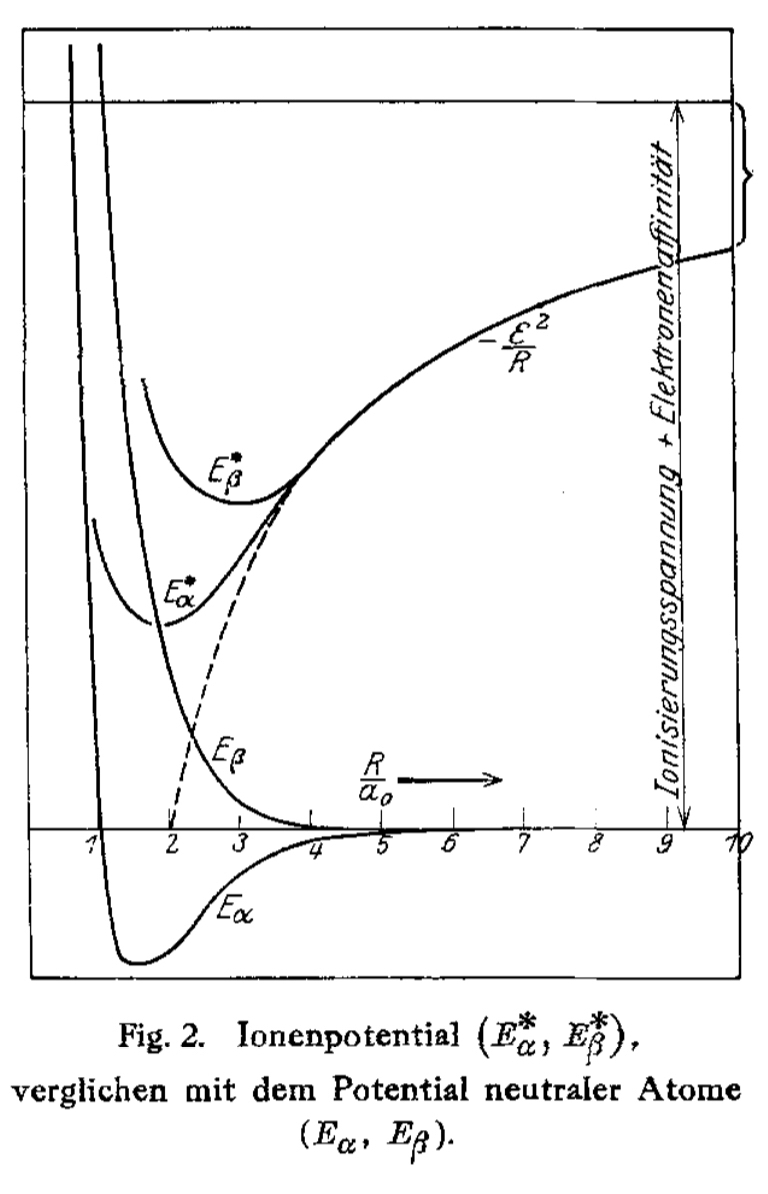
\includegraphics[width=0.5\textwidth]{fig2}
%	\end{center}
\end{wrapfigure}

As the two ions approach one another the associated eigenvalues $E_\alpha^*$ and $E_\beta^*$ initially decrease, roughly as the ionization potential $-\frac{\varepsilon^2}{R}$ (figure 2). Here, $E_\alpha^*$, associated to the nodeless $\alpha^*$, is always lower than $E_\beta^*$. The difference $E_\beta^* - E_\alpha^*$ is proportional to the frequency of the exchange of ion charges.

As long as the eigenvalues $E_\alpha^*$ and $E_\beta^*$ do not come into the vicinity of our energy curves of \S2 (they are again marked in figure 2\footnote{On the grounds of the subsequent considerations we give preference to the here-specified assignment of the terms proposed by F. Hund, l.c., Fig. 12, since it emerges from the considerations of \S4 that not all states of the $2-\H$ problem go over to the $\H_2$ problem, not to mention those of \He.}), \?{the calculations of \S1 are to be interpreted as perturbations of the eigenvalue $2E_0=-27\unit{Volt}$ and are not objectionable}{sind die Rechnungen des \S1 als Störungen des Eigenwertes $2E_0 = -27\unit{Volt}$ aufzufassen und nicht zu beanstanden}. But something new happens when the new curves come very close to the old. For this value of $R$ the associated eigenvalue will become \?{multi-valued}{mehrfach}, there will be degeneracy, the "correct" zero-order eigenfunctions will then become certain linear combinations of the eigenfunctions at the point of intersection, which yields a secular problem. The calculations of \S1 would then be problematic if they would yield different linear combinations in this situation than used there. We will now prove this.

\subsection{} First, $E_\alpha^*$ and eventually also $E_\beta^*$ cross the upper of the two energy curves $E_\beta$. Since $\alpha^*$ and $\beta^*$ are symmetric, while $\beta$ is antisymmetric in 1 and 2, and because of the symmetry of the differential equation in 1 and 2 even with arbitrarily larger perturbations this symmetry behavior will not be lost, so the matrix elements of the "perturbation energy"\footnote{On this function $H$ see the discussion is \S3.} $H$ which occurs in the secular problem
\uequ{
\int H\alpha^*\beta\d\tau_1\,\d\tau_2 &= 0,\\
\int H\beta^*\beta\d\tau_1\,\d\tau_2 &= 0
}
vanish.

The secular problem at the intersection of $E_\alpha^*$ with $E_\beta$ then reads
\uequ{
\left|\begin{matrix}
	\int H{\alpha^*}^2\d\tau - E & 0\\
	0 & \int H\beta^2\d\tau - E 
\end{matrix}\right| =0.
}

A secular problem of the same type is obtained for the intersection $E_\beta^2$ with $E_\beta$. From this it arises that the secular eigenvalues of these are like the original, and in addition, that the eigenfunctions come through \?{unmixed}{unvermengt}, without forming linear combinations\footnote{This \?{unmixedness}{Unvermengbarkeit} of $\beta$ with $\alpha^*$ and $\beta^*$ can be put forward more physically, since $\beta$ have parallel spins, $\alpha^*$ and $\beta^*$ (namely, symmetric \He ground state configurations!) have unequal spins; if the configuration $\beta$ exists between two atoms, then it cannot simultaneously be $\alpha^*$ or $\beta^*$. A linear combination of $\beta$ with $\alpha^*$ or $\beta^*$ would be totally incomprehensible.}.

\subsection{} So then \?{$\alpha^*$ is in conflict with $\alpha$}{wird $\alpha^*$ sich mit $\alpha$ auseinanderzusetzen haben}. If only the ion potential $-\frac{\varepsilon^2}{R}$ is taken into account, then $E_\alpha^*$ would cross the \?{null axis}{Nullachse} at $R=2a_0$ (figure 2, dashed curve). But in this region one is already well within the charge cloud (it is much more dispersed for $H^-$ than for $H$) and consequently the ionization attraction will gradually cease and give way to a repulsion there\footnote{The presence of an ionic repulsion for smaller distances (on the basis of the quantum-mechanical charge distribution) has already been independently noted by L. Pauling, Proc. Roy. Soc. (A) 114, 181, 1927 and A. Unsöld, ZS. f. Phys. (at press).}. It is easily seen that by considering the exchange terms, the two curves $E_\alpha^*$ and $E_\alpha$ remain distant in the vicinity of the minimum of $E_\alpha$ (figure 2, the solid curve $E_\alpha^*$ is only very qualitative.) The linear combination of $\alpha$ with $\alpha^*$ is accordingly still very weak in the vicinity of $R=a_0$ -- it can be interpreted as a perturbation of the eigenfunction $\alpha$. Calculating $E_\alpha$ without considering the linear combination with $E_\alpha^*$ is justified, and for just this reason it is characterized as "primarily homopolar”. For its part, $E_\alpha^*$ likewise has a minimum somewhere; at this location there would then be room for a polar molecule. But insofar as this minimum is not an absolute minimum, and insofar as it can be taken over to the known absolute minimum on an adiabatic\footnote{The word "adiabatic" is not totally appropriate here, since the transfer goes through a point of degeneracy.} path, one is justified in saying that the polar molecule formation does nor represent the stable configuration of the two \El{H} atoms in the molecule.  In a separation of the molecule without simultaneous excitation one will expect to find two neutral atoms with greater probability. How the two solutions $\alpha$ and $\alpha^*$ linearly combine cannot be foreseen without in-depth examination.

\WTF{???} \?{Finally, on grounds of the same considerations as above, the unperturbed  $\beta^*$ solution (antisymetric in $\psi$ and $\varphi$) would enforce the  $\alpha$ solution.}{Die Lösung $\beta^*$ schließlich (antisymmetrisch in $\psi$ and $\varphi$) würde ungestört die Lösung $\alpha$ auf Grund derselben Überlegungen wie oben durchsetzen.} But, that probably does not happen. In molecule formation, $\beta^*$ plays no part because of its non-transferrability into a \El{He} configuration -- it has a node between the nuclei.

We would like to believe that the categories of degeneracy and symmetry behavior put forward here might be typical for a wide range of facts which are connected with the interaction of atomic systems upon one another, above all with the discontinuities of their types of chemical behavior\footnote{One can wonder whether the exchange phenomena, which are so decisive for the interactions of atoms, are being noticed in other areas of physics. We would like to indicate two here. In collision processes, the exchange of colliding and atomic electrons brings with it the possibility of also exciting quantum jumps between optically-non-combining term systems (e.g. $1{{}^1 S}--2{{}^3S}$ in helium). According to the Born theory, such transitions are only possible on grounds of minimal magnetic interaction. In the interpretation of the force laws of atomic nuclei that become apparent in the scattering experiments with $\alpha$ or \El{H} particles, one must take account of the exchange of \?{nuclear particles}{Kernbaustein} as an essential influence.}.

We would like to give heartfelt thanks to Herrn Prof. Schrödinger for the kind, solicitous interest with which he has followed our work. We thank the International Education Board for making it possible for us to work here in Zurich.

Zurich, Physics institute of the University, June 1927. 



\end{paper}